\section{作业及答案：结构力学基础与技巧班第11次作业及答案（力法2）}
\begin{analysisbox}
高阶超静定力法要注意未知量编号、柔度矩阵对称性和自由项符号。解出多余力后，将基本体系内力与各单位多余力内力线性叠加。
\end{analysisbox}
\subsection*{第 1 页转写}
叫研究生入学考试辅导丛书结构力学（第二版）

EA

C

q勹B

G 1』

20kN

IF

丫G

y

A

7?7?77' 玉

j\_

2

尸

B

＼

L

L

6m

 

6m

l

1

，

1

,

,

．，

图5-149

图5-150

4. 弹性支承超静定结构的计算

5-31 图5-153 (a)所示结构，取图5 - 153 (b)为力法基本体系，其力法典型方程

为(

)。k为弹簧刚度。（中南大学2012)

Fp

，

a

十

图5-151

a

一。

一

20kN

I

EA==

\{

3m

\{

l

r

k-

(a)

(b)

图5-152

图5-153

5-32 求图5-154所示结构在给定基本体系下的力法方程及方程中的所有系数。（青

岛理工大学2008)

5-33试计算图5-155所示具有弹性支座的结构，并作弯矩图。抗转刚度系数ko =

單（中国矿业大学2008)

q

q

贮I I I

I I I I

贮A

\textbackslash{}

u

j

C

EI

EI

I

］

ko

M

El嘴数

k

\{

lr-3El/13

＼

1-

f

I

112

I

//2

图5-154

图5-155

5. 支座发生位移和温度变化时超静定结构的计算

5-34 图5-156中等EI值单跨梁两侧温度变化时，M图位千（

）。（青岛理工大

232
\begin{figure}[H]\centering
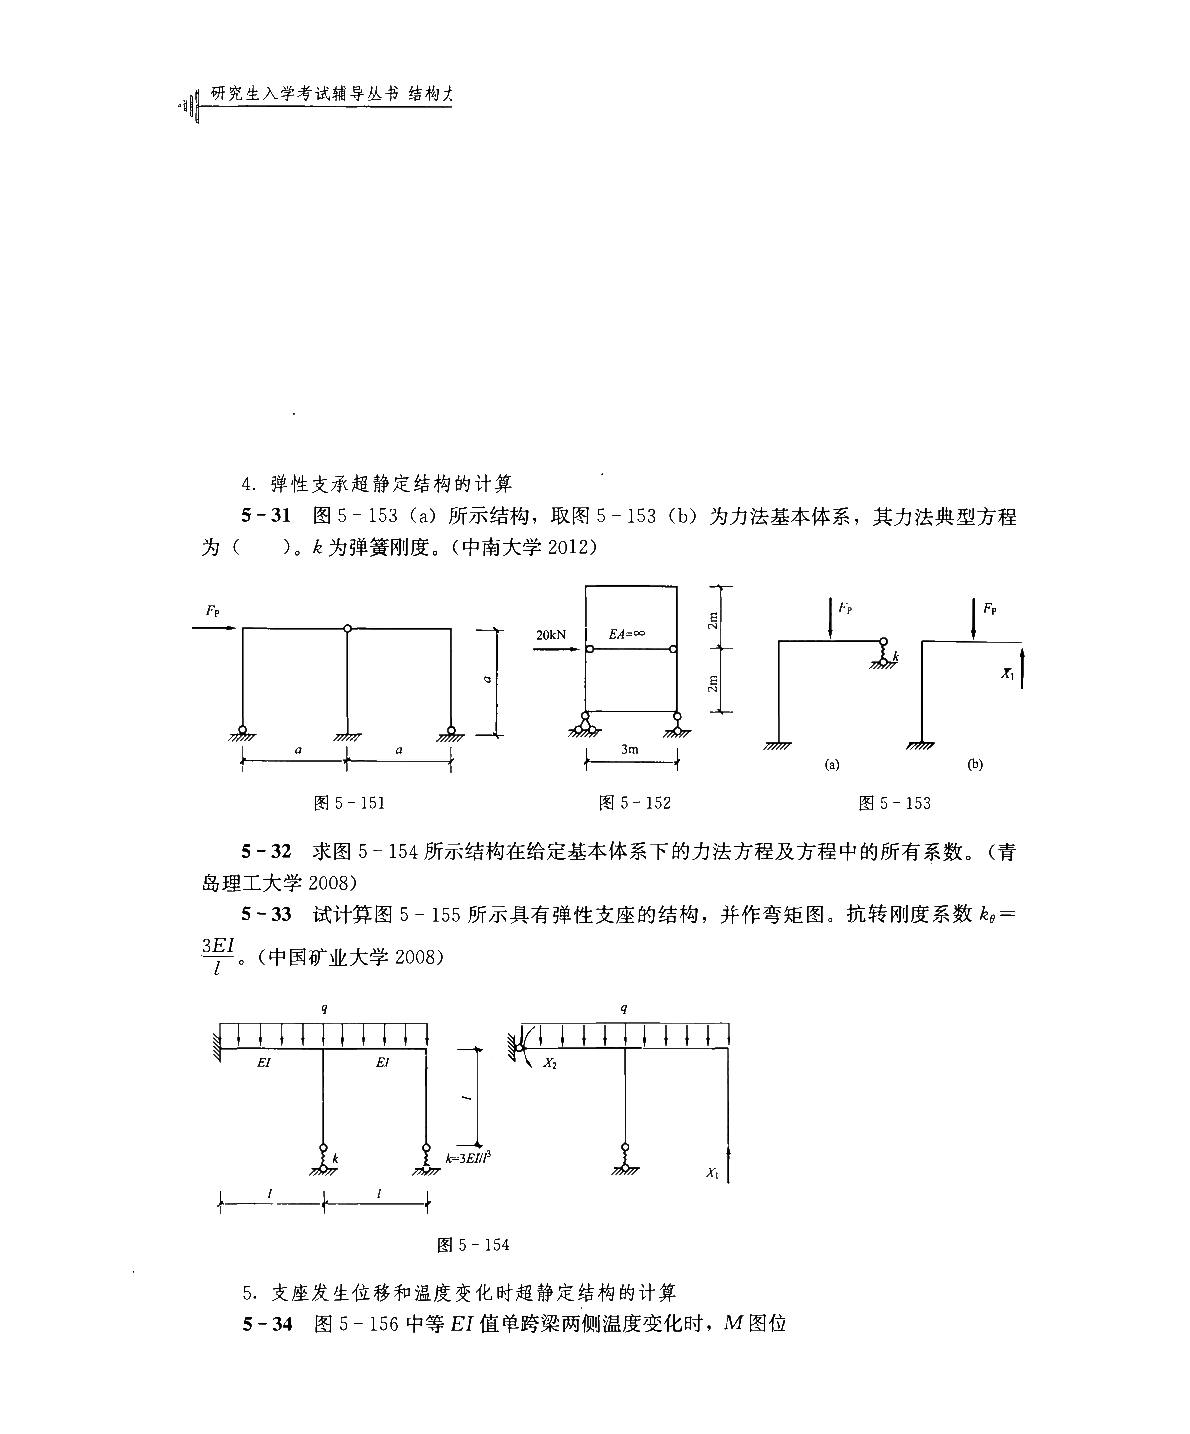
\includegraphics[width=0.92\textwidth]{figures/src14_p001.jpg}
\caption{结构力学基础与技巧班第11次作业及答案（力法2） 第 1 页清理图形页}
\end{figure}
\subsection*{第 2 页转写}
学2008)

A.低温侧

B.高温侧

C. 不同侧

D.零

[01X+012X2+A1c=,

5 - 35

判断题。取图5-157所示结构基本体系，则力法方程为

021X+022X2+2c=2

[41c=0

）（福州大学2011)

4=-6

5 - 36

图5-158所示刚架除承受荷载外，支座A下沉了$\triangle$=2cm，且顺时针转动了Q=

0.01rad。已知E=2.1$\times$10*kN/cm ，I=2000cm*，用力法求此刚架的弯矩图。（华南理工

大学2009)

X2

50kN

+2r 

+rC

(b)

(a)

4m

图5-156

图5-157

图5-158

6.超静定结构的位移计算

5-37图5-159所示梁（跨长1）支座位移产生的跨中点竖向位移为（

)。（哈尔

滨工业大学2011)

A. lp/16

B. lp/8

C. lp/4

D. lp/2

5-38图5-160所示为计算得到的超静定刚架的弯矩图，则C点的角位移pc=

，E点的水平位移$\triangle$HE=

（湖南大学2011）

5-39图5-161所示一端固定、另一端定向支承的等截面梁，当A端发生单位转角

0=1时，B端的竖向位移$\triangle$=

，（重庆大学2010）

111.98

7.29

3.65

EI

8.33

1.04

2EI

EI

0-1

3.65

F0.52

4.17

M图(x0.01Fp)

图5-159

图5-160

图5-161

5-40

图5-162所示结构，各杆抗弯刚度EI为常数，忽略杆件的轴向变形。（1）根
\begin{figure}[H]\centering
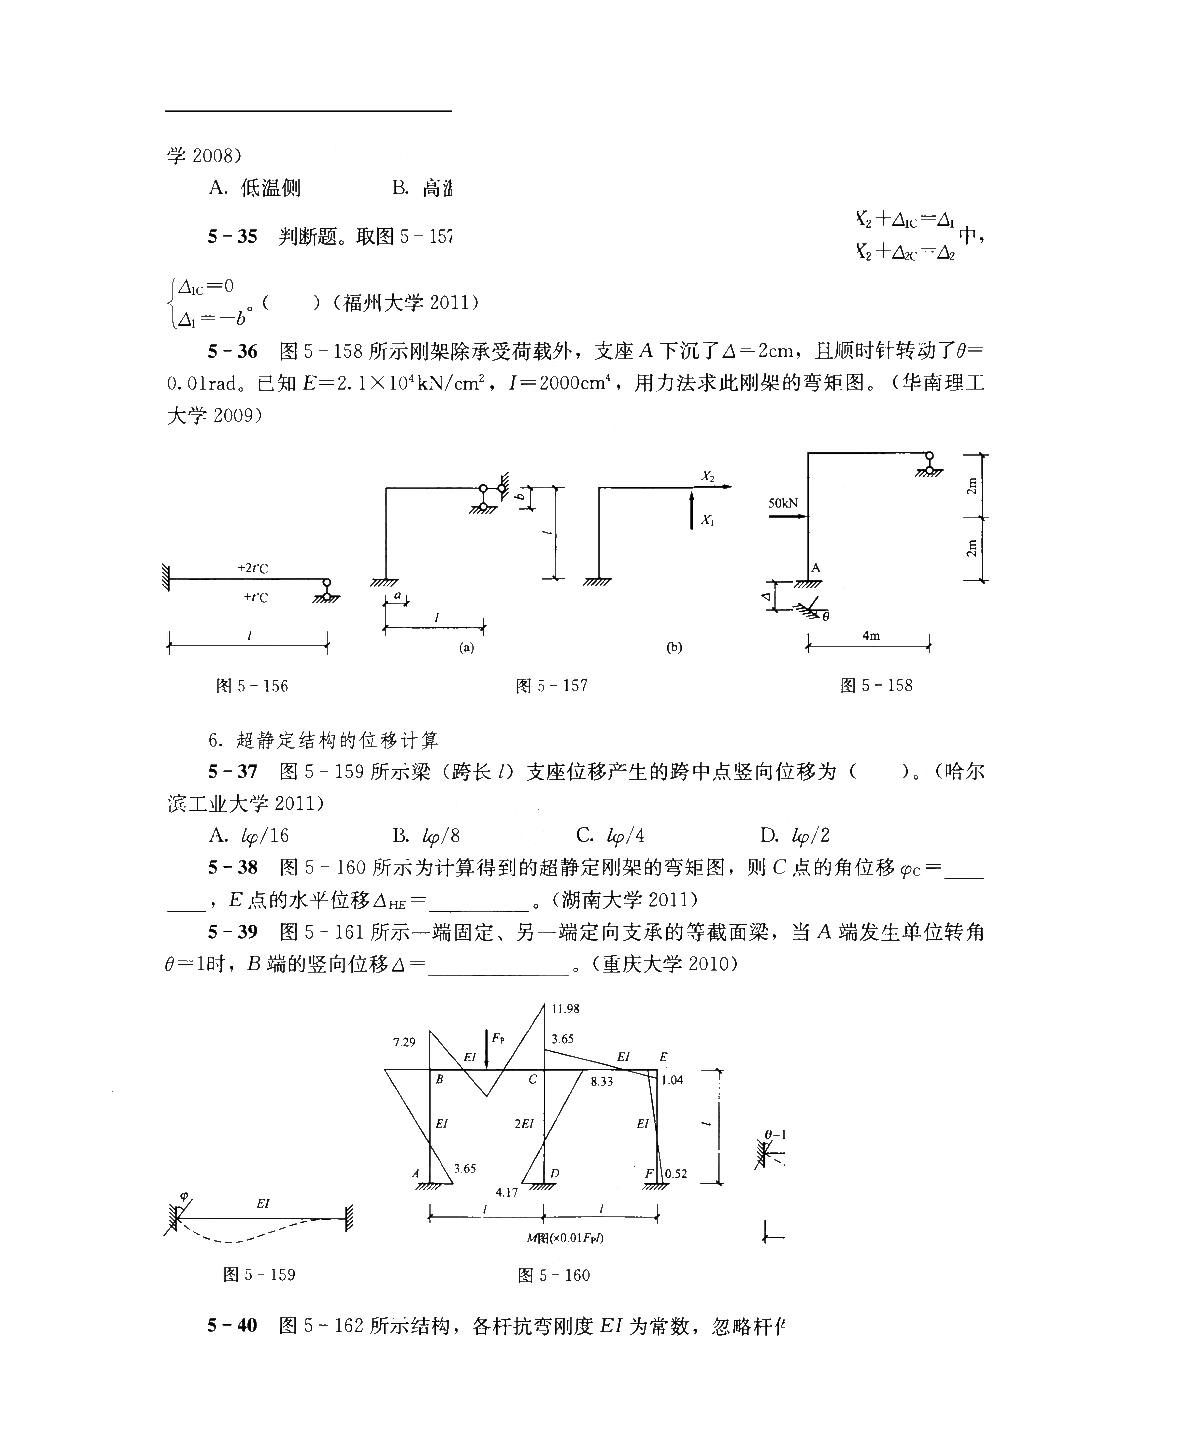
\includegraphics[width=0.92\textwidth]{figures/src14_p002.jpg}
\caption{结构力学基础与技巧班第11次作业及答案（力法2） 第 2 页清理图形页}
\end{figure}
\subsection*{第 3 页转写}
研究生入学考试辅导丛书结构力学（第二版）

据结构与荷载的特点，选用最简便的方法作刚架的弯矩图；（2）求C点的水平位移。（武汉

理工大学2011)

10kN

20kN-m

2m

2m

2m

图5-162

234
\begin{figure}[H]\centering
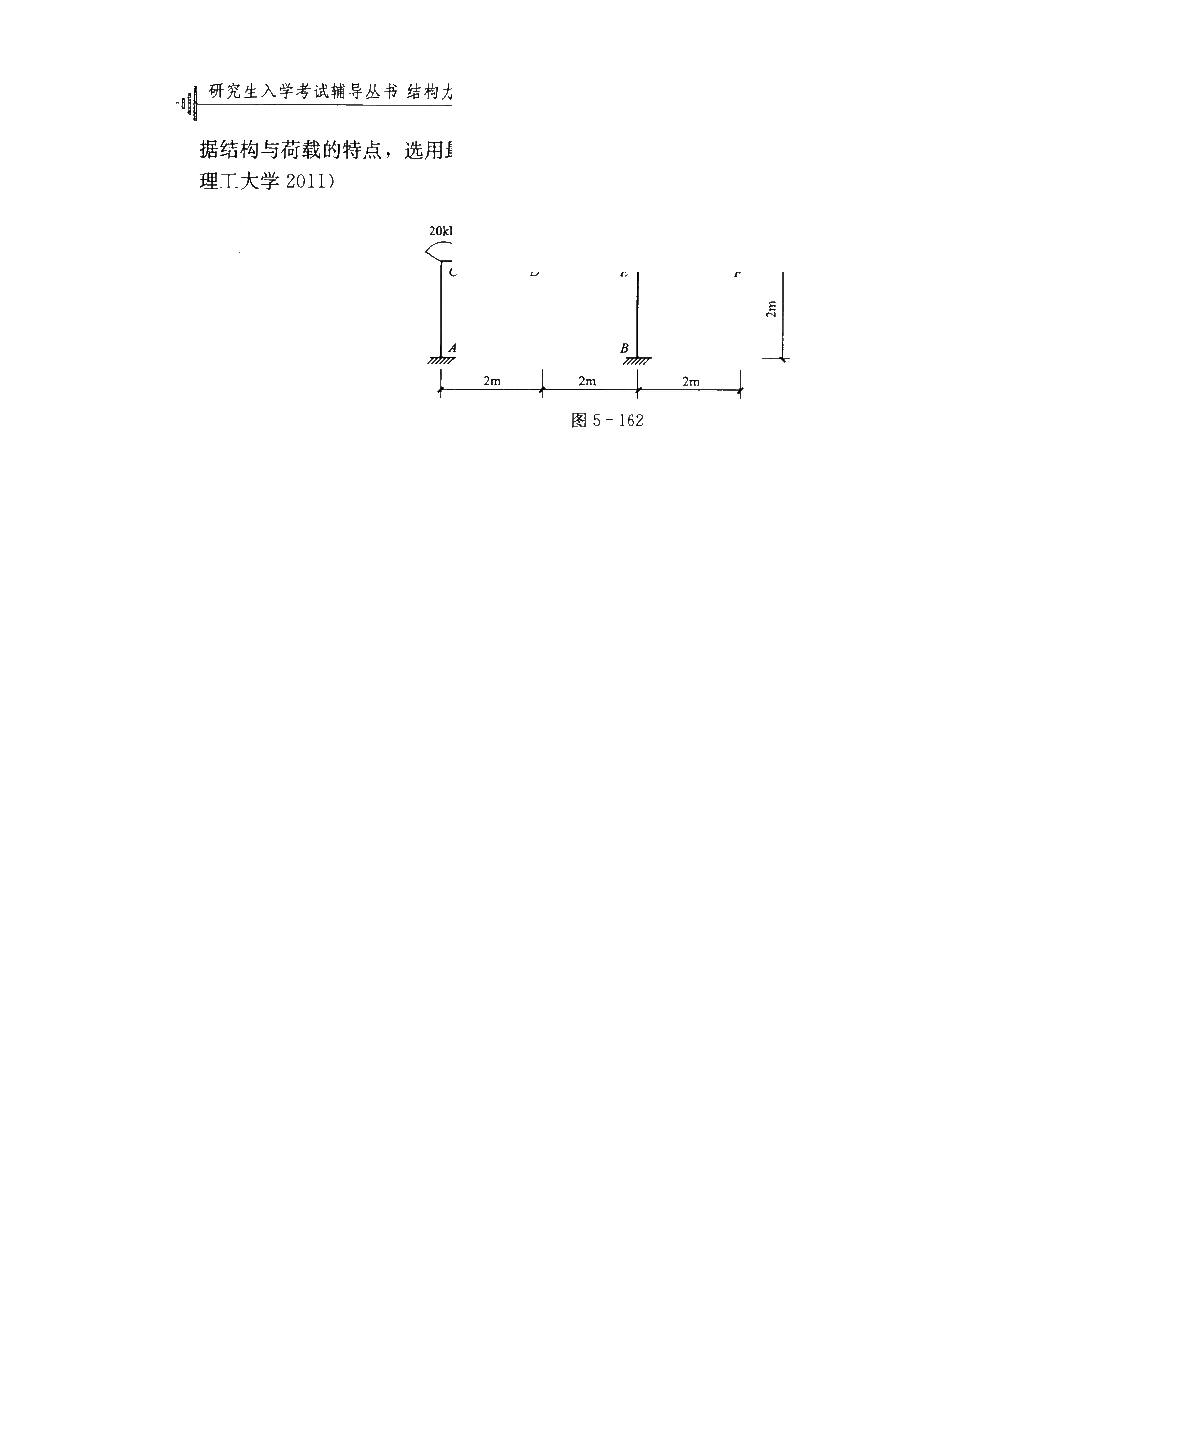
\includegraphics[width=0.92\textwidth]{figures/src14_p003.jpg}
\caption{结构力学基础与技巧班第11次作业及答案（力法2） 第 3 页清理图形页}
\end{figure}
\subsection*{第 4 页转写}
5-32、

(27
\begin{figure}[H]\centering
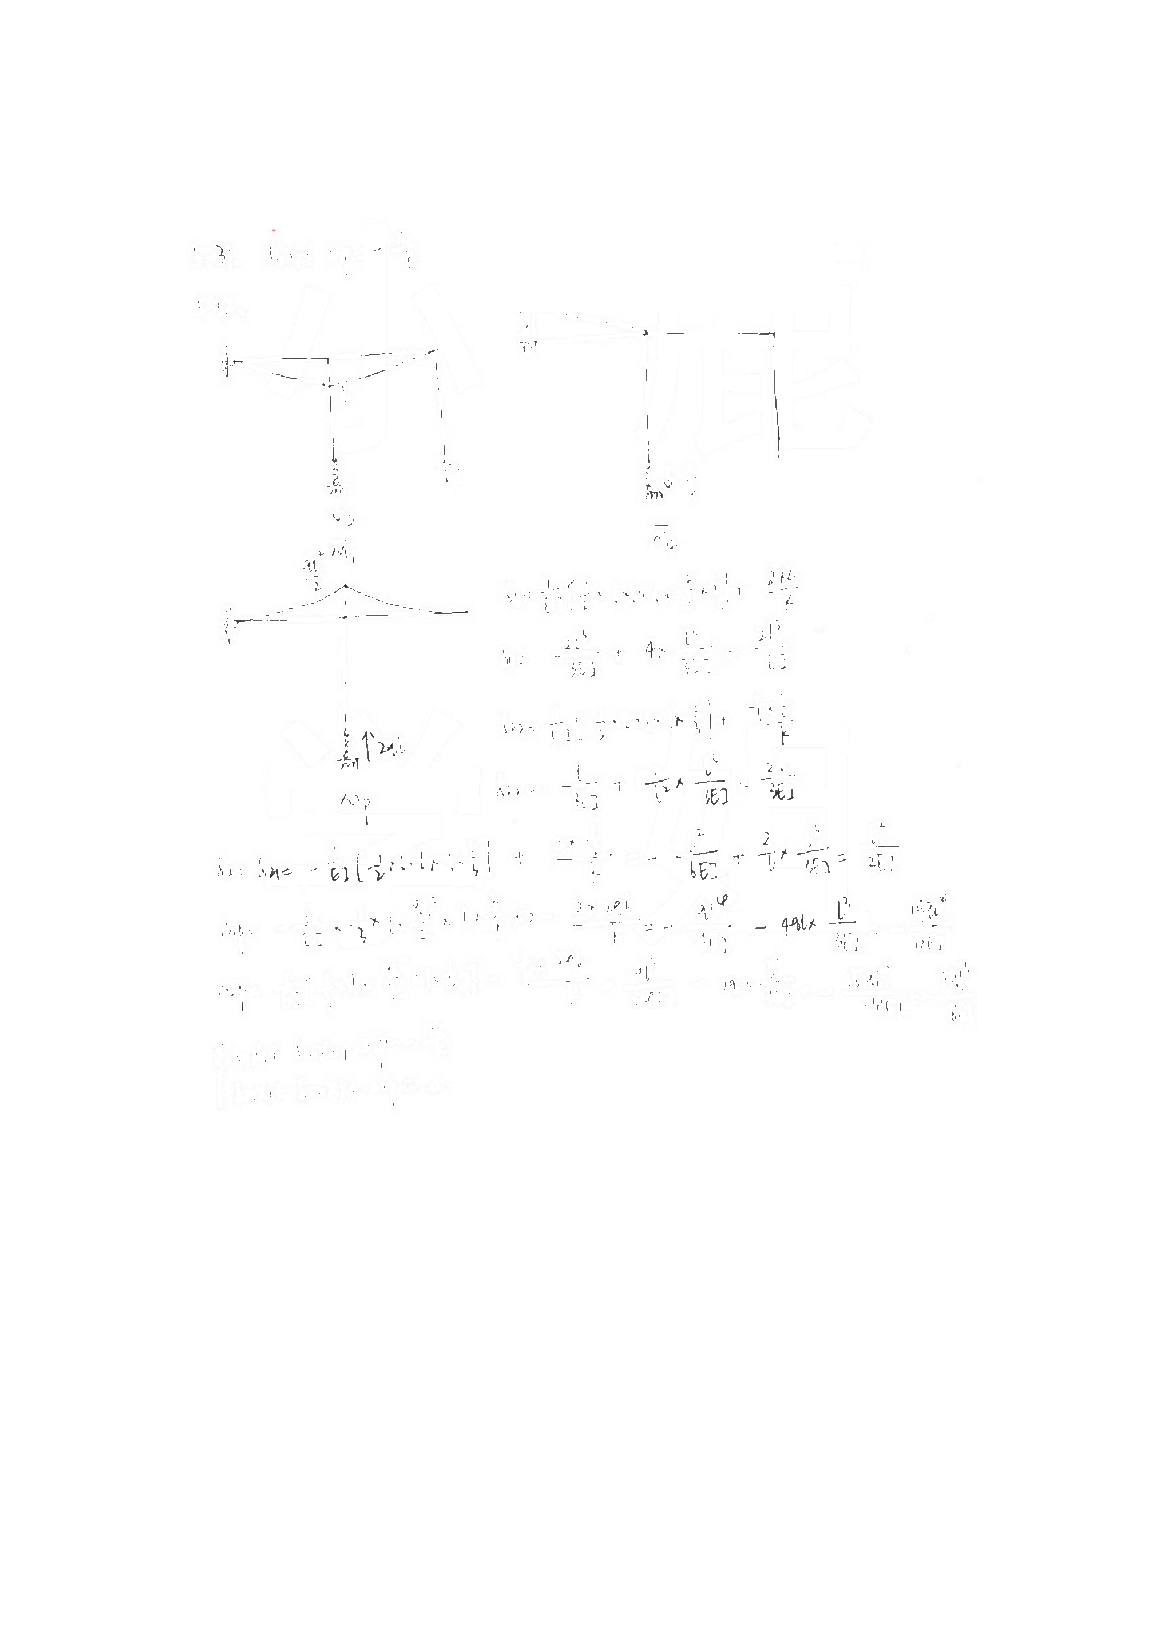
\includegraphics[width=0.92\textwidth]{figures/src14_p004.jpg}
\caption{结构力学基础与技巧班第11次作业及答案（力法2） 第 4 页清理图形页}
\end{figure}
\subsection*{第 5 页转写}
5-33

gml1

12-

Snxitbp=-

XL

1个
\begin{figure}[H]\centering
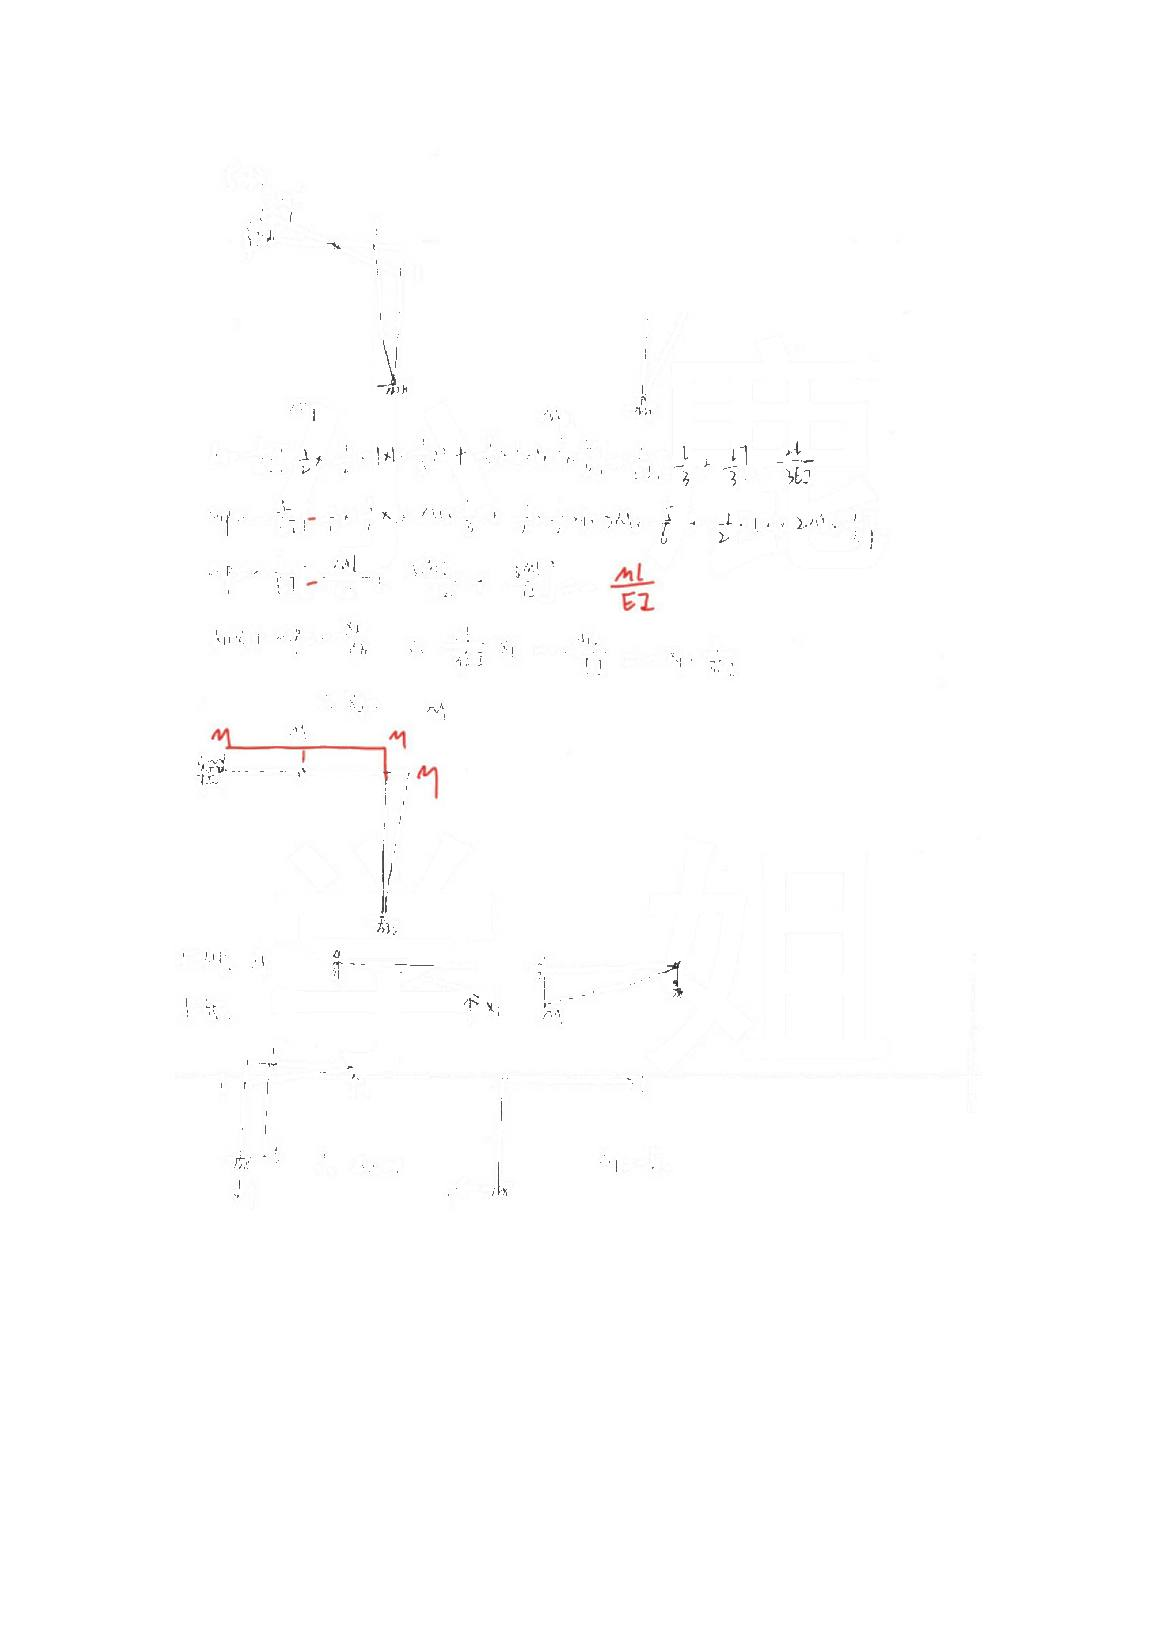
\includegraphics[width=0.92\textwidth]{figures/src14_p005.jpg}
\caption{结构力学基础与技巧班第11次作业及答案（力法2） 第 5 页清理图形页}
\end{figure}
\subsection*{第 6 页转写}
b1L=-006m

ixbnt

X1-7.6p w
\begin{figure}[H]\centering
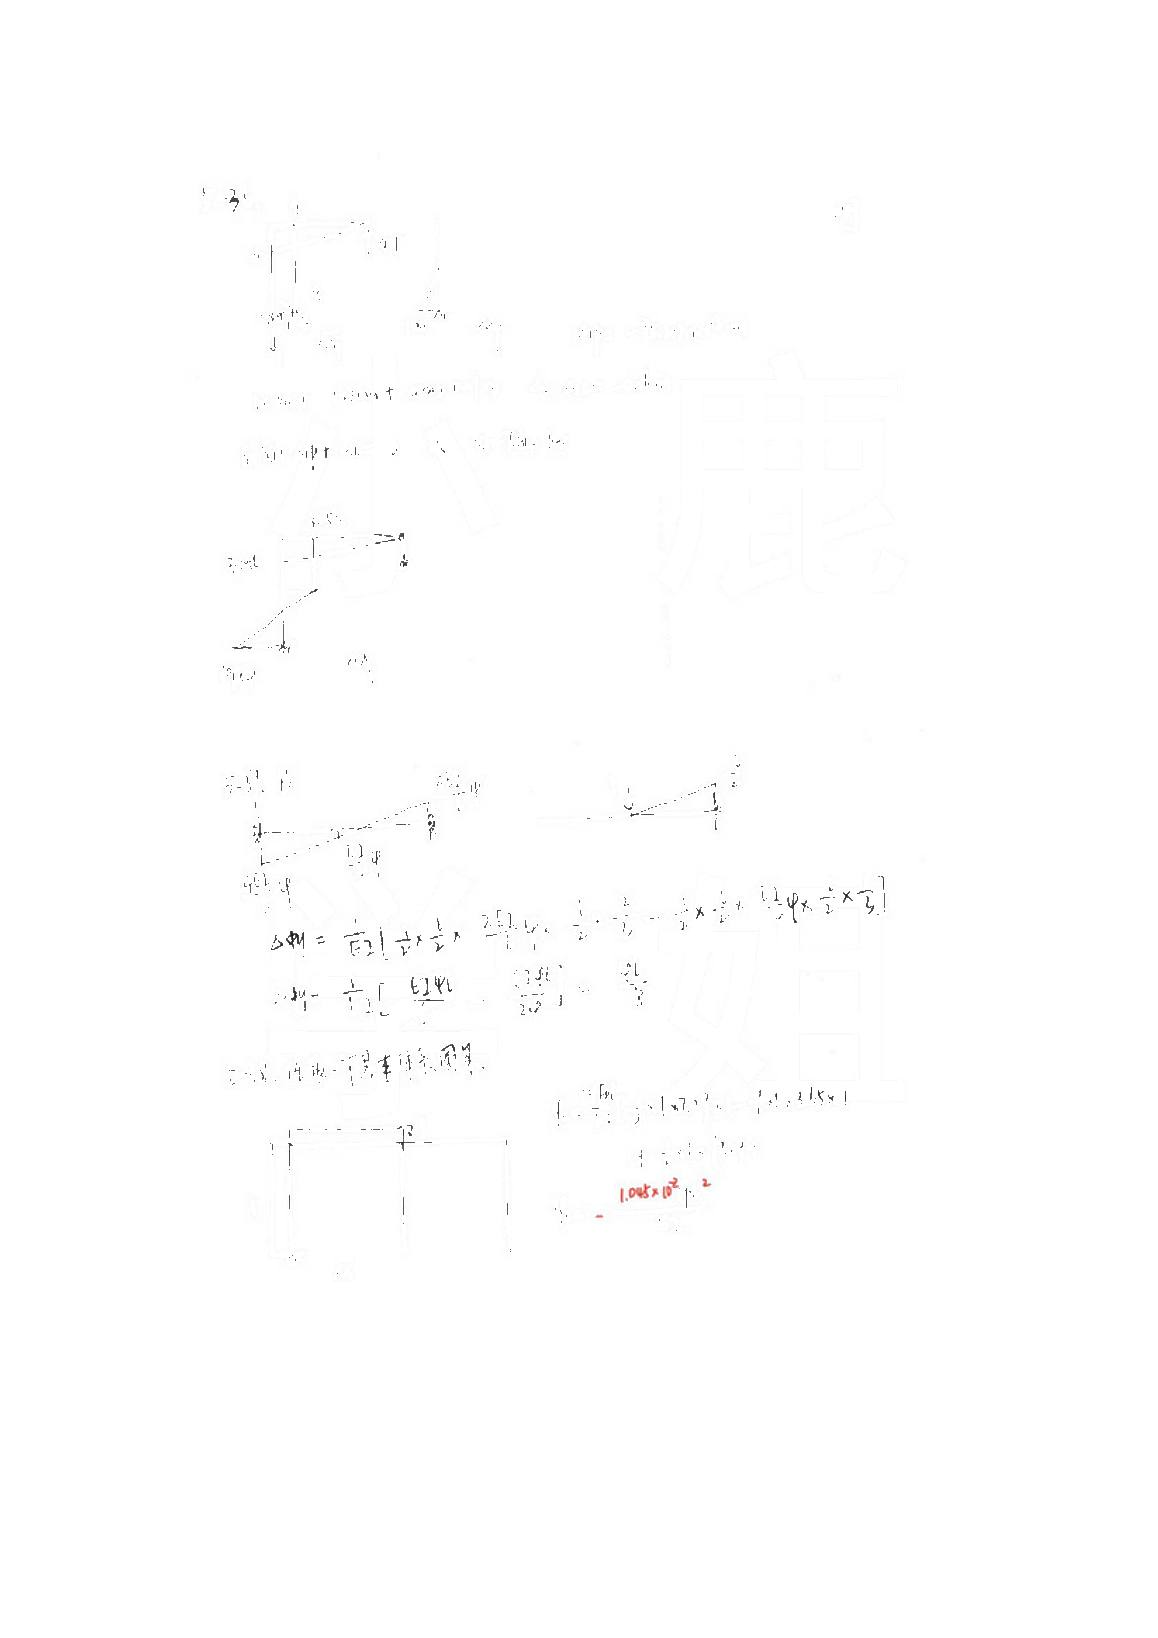
\includegraphics[width=0.92\textwidth]{figures/src14_p006.jpg}
\caption{结构力学基础与技巧班第11次作业及答案（力法2） 第 6 页清理图形页}
\end{figure}
\subsection*{第 7 页转写}
415--167+105FL

5- L0. (1)

roky.m

[2x]
\begin{figure}[H]\centering
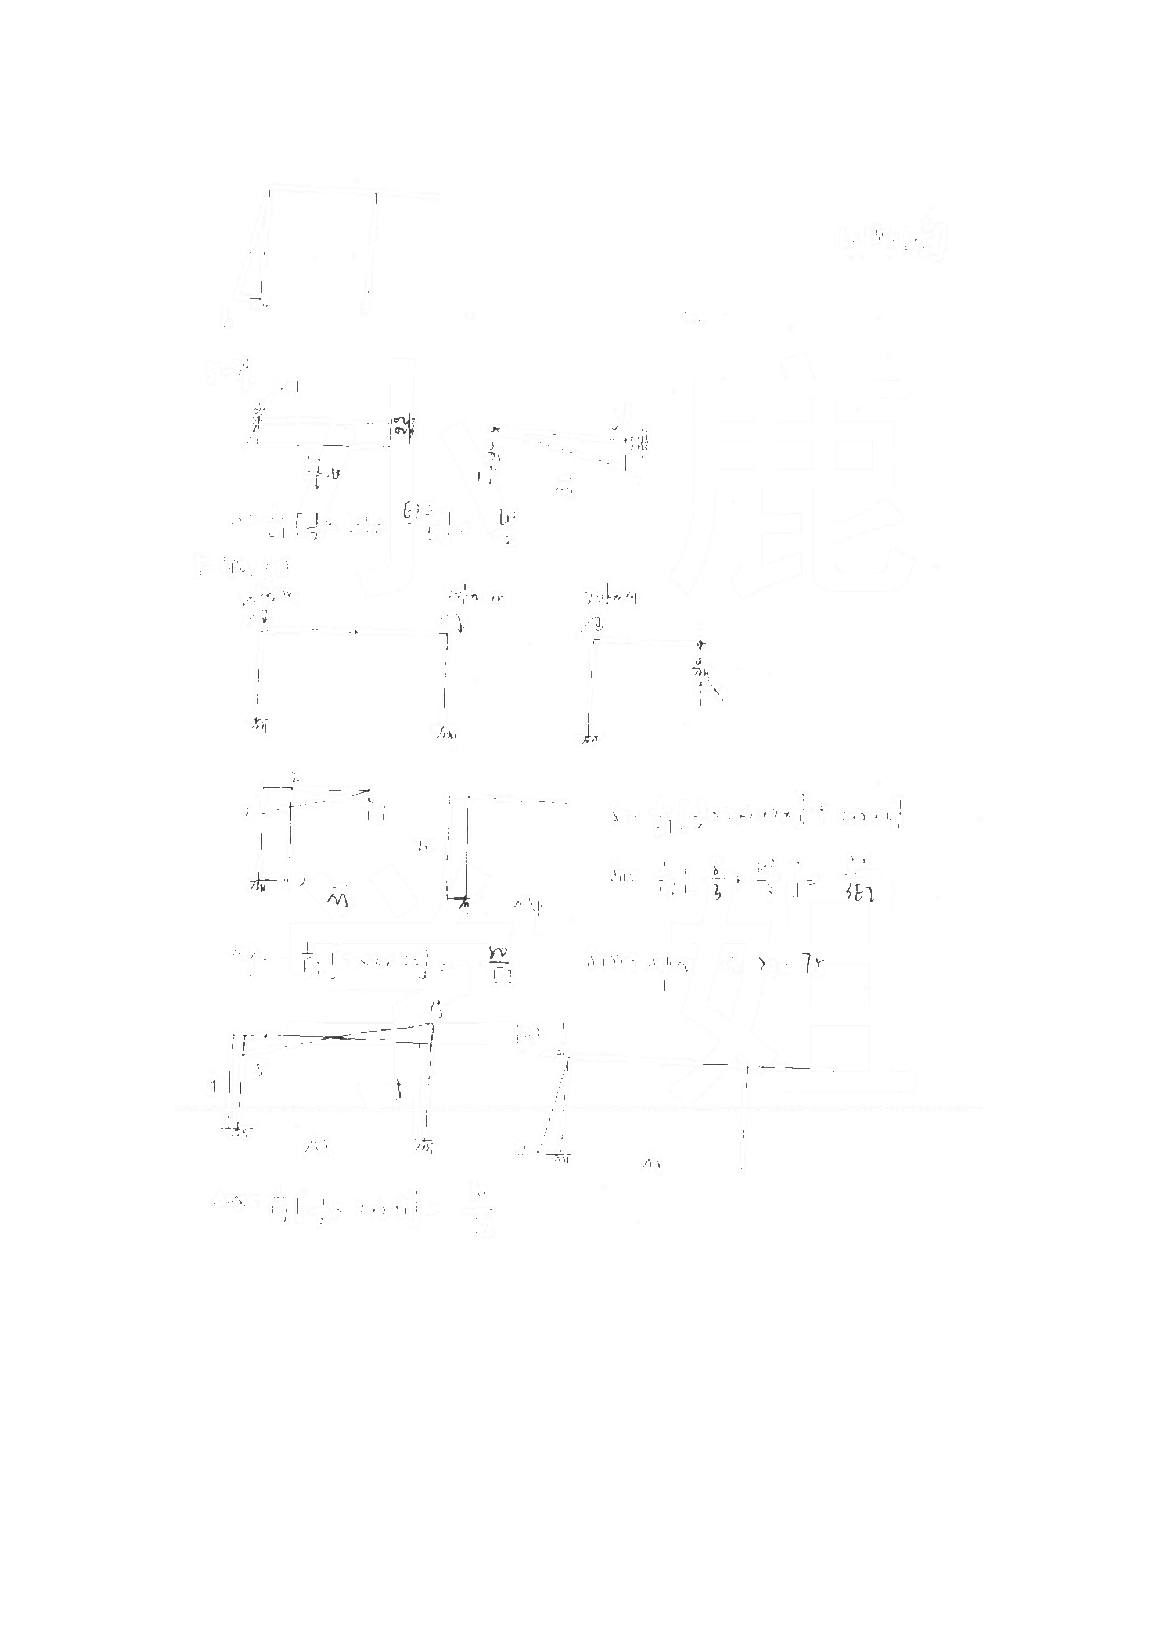
\includegraphics[width=0.92\textwidth]{figures/src14_p007.jpg}
\caption{结构力学基础与技巧班第11次作业及答案（力法2） 第 7 页清理图形页}
\end{figure}
\subsection*{第 8 页转写}
研究生入学考试辅导丛书结构力学（第二版）

据结构与荷载的特点，选用最简便的方法作刚架的弯矩图；（2）求C点的水平位移。（武汉

理工大学2011)

10kN

20kN-m

2m

2m

2m

图5-162

234
\begin{figure}[H]\centering
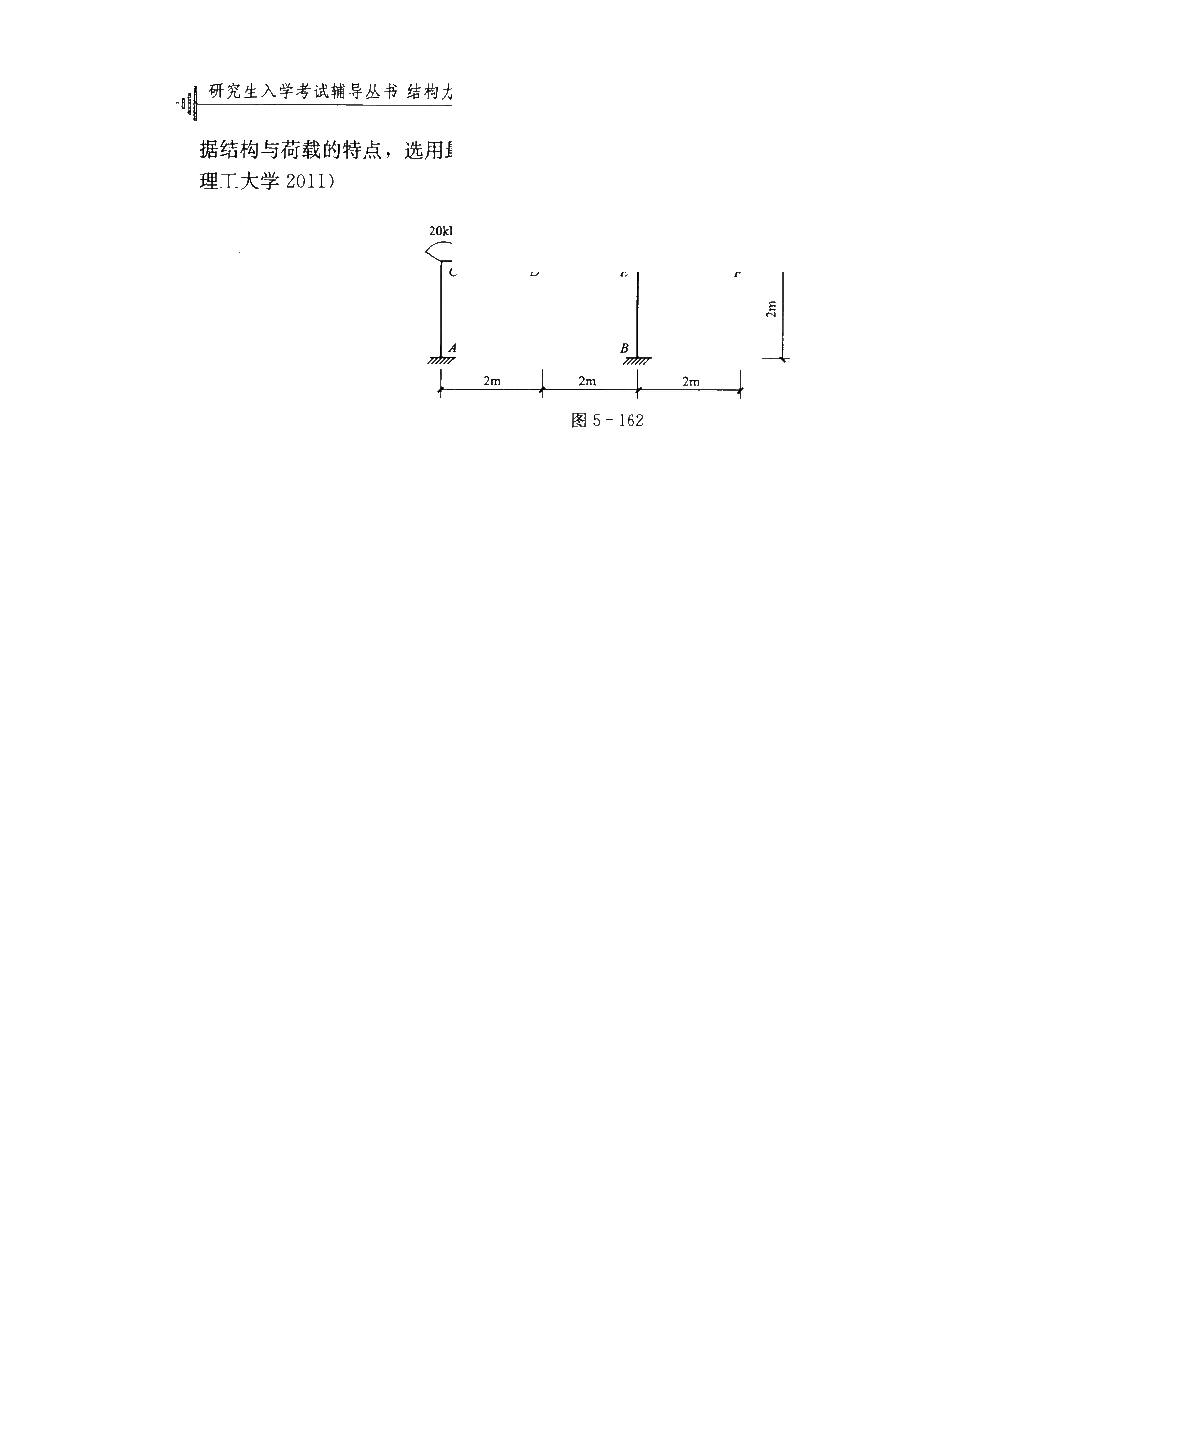
\includegraphics[width=0.92\textwidth]{figures/src14_p008.jpg}
\caption{结构力学基础与技巧班第11次作业及答案（力法2） 第 8 页清理图形页}
\end{figure}
